\providecommand{\curso}{Séptimo Básico}
\providecommand{\colegio}{Colegio Divina Pastora}
\providecommand{\tituloDocumento}{Guía 3}
\providecommand{\subtituloDocumento}{Tabla de frecuencias (\# 2)}
\providecommand{\tituloItem}{Parte}
\documentclass{cdplf-prueba}
\begin{document}
\subsection{}

Use los datos a continuación para llenar la tabla de frecuencias.

\underline{Datos:} \hspace{4pt} 10 \hspace{4pt}\textbullet\hspace{4pt} 10 \hspace{4pt}\textbullet\hspace{4pt} 13 \hspace{4pt}\textbullet\hspace{4pt} 12 \hspace{4pt}\textbullet\hspace{4pt} 15 \hspace{4pt}\textbullet\hspace{4pt} 23 \hspace{4pt}\textbullet\hspace{4pt} 8 \hspace{4pt}\textbullet\hspace{4pt} 10 \hspace{4pt}\textbullet\hspace{4pt} 8 \hspace{4pt}\textbullet\hspace{4pt} 17 \hspace{4pt}\textbullet\hspace{4pt} 15 \hspace{4pt}\textbullet\hspace{4pt} 7 \hspace{4pt}\textbullet\hspace{4pt} 13 \hspace{4pt}\textbullet\hspace{4pt} 12 \hspace{4pt}\textbullet\hspace{4pt} 12 \hspace{4pt}\textbullet\hspace{4pt} 14 \hspace{4pt}\textbullet\hspace{4pt} 10 \hspace{4pt}\textbullet\hspace{4pt} 7 \hspace{4pt}\textbullet\hspace{4pt} 10
\begin{center}\begin{tblr}{colspec={ccccc},hlines,vlines,hline{2,Z} = {1}{-}{},hline{2,Z} = {2}{-}{},row{even}={black!10},rowsep=0pt}
  .&Frecuencia&Probabilidad&Frecuencia Acumulada&Probabilidad Acumulada \\
 7&&&& \\
 8&&&& \\
 10&&&& \\
 12&&&& \\
 13&&&& \\
 14&&&& \\
 15&&&& \\
 17&&&& \\
 23&&&& \\
 \end{tblr}\end{center}
\subsection{}

Haga un gráfico de barras usando las frecuencias de la tabla anterior.
\begin{center}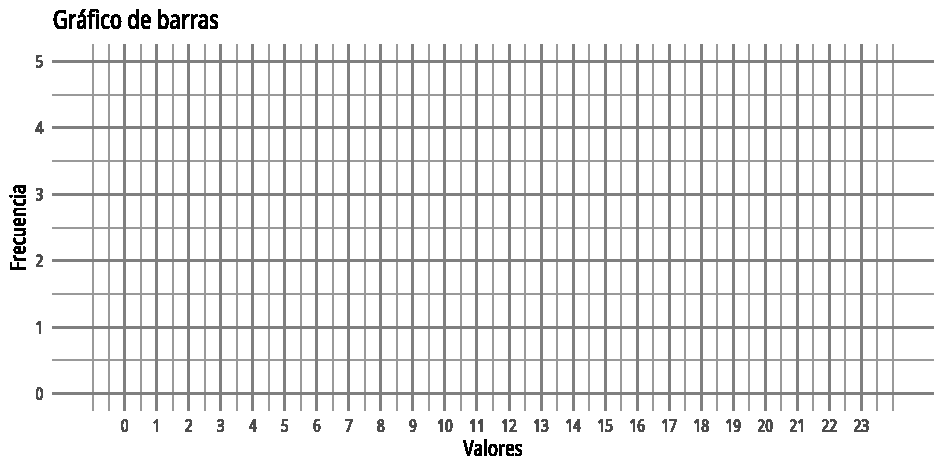
\includegraphics{grafico_vacio_2.pdf}\end{center}

\subsection{}
Usando los resultados anteriores, responda las siguientes preguntas
\begin{tasks}[label={\tcbox[colback=black!60, colframe=black!60, coltext=white, on line, boxsep=0pt, left=3pt, right=3pt, top=2pt, bottom=2pt]{\sffamily\bfseries\alph*}},
item-indent=1.2cm,column-sep=20pt,label-offset=0.3cm,label-width=15pt,after-item-skip=10pt]
    \task! ¿Cuánto vale la media (promedio) de los datos? ¿Qué significa que tenga este valor? \begin{lineas}[height=1.5cm]\end{lineas}
    \task! ¿Cuánto vale la mediana de los datos? ¿Qué significa que tenga este valor? \begin{lineas}[height=1.5cm]\end{lineas}
    \task! ¿Cuál es el rango de los datos? ¿Qué significa que tenga este valor? \begin{lineas}[height=1.5cm]\end{lineas}
    \task! ¿Cuánto vale el primer cuartil de los datos? ¿Qué significa que tenga este valor? \begin{lineas}[height=1.5cm]\end{lineas}
    \task! ¿Cuánto vale el tercer cuartil de los datos? ¿Qué significa que tenga este valor? \begin{lineas}[height=1.5cm]\end{lineas}
    \task! ¿A qué valor corresponde el percentil del 90\%? ¿Qué significa que tenga este valor? \begin{lineas}[height=1.5cm]\end{lineas}
\end{tasks}
\subsection{}

Haga un diagrama de caja usando los datos anteriores.
\begin{center}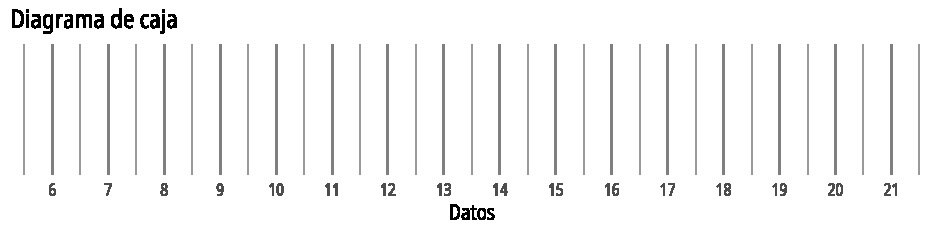
\includegraphics{diagrama_caja_vacio_2.pdf}\end{center}

\newpage\section*{Soluciones}
\setcounter{subsection}{0}
\subsection{}

\begin{center}\begin{tblr}{colspec={ccccc},hlines,vlines,hline{2,Z} = {1}{-}{},hline{2,Z} = {2}{-}{},row{even}={black!10}}
  .&Frecuencia&Probabilidad&Frecuencia Acumulada&Probabilidad Acumulada \\
 7&2&0.105&2&0.105 \\
 8&2&0.105&4&0.21 \\
 10&5&0.263&9&0.473 \\
 12&3&0.158&12&0.631 \\
 13&2&0.105&14&0.736 \\
 14&1&0.053&15&0.789 \\
 15&2&0.105&17&0.894 \\
 17&1&0.053&18&0.947 \\
 23&1&0.053&19&1 \\
 \end{tblr}\end{center}
\subsection{}
\begin{center}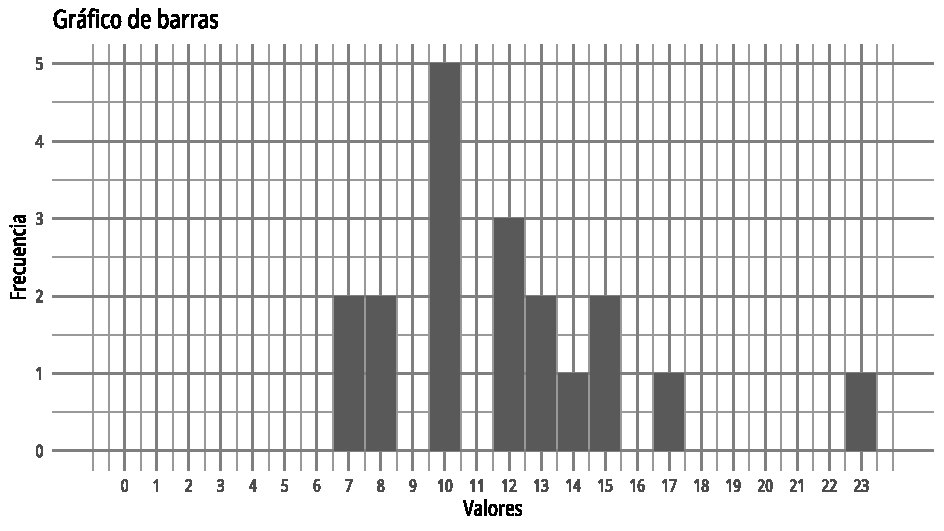
\includegraphics{grafico_barras_2.pdf}\end{center}
\subsection{}
\begin{tasks}[label={\tcbox[colback=black!60, colframe=black!60, coltext=white, on line, boxsep=0pt, left=3pt, right=3pt, top=2pt, bottom=2pt]{\sffamily\bfseries\alph*}},
item-indent=1.2cm,column-sep=20pt,label-offset=0.3cm,label-width=15pt,after-item-skip=10pt,item-format=\raggedright](2)\task La media es 11.895.
 Esto significa que los valores más frecuentes son los que están cercanos a 11.895, y es donde también se encuentran las barras más altas 
 en el gráfico de barras.\task La mediana es 12. 
 Esto significa que la mitad (50\%) de los datos tiene un valor menor 
 o igual a 12.\task El rango de los datos es 16. Esto 
 significa que la distancia entre el máximo (23) y el mínimo (7) de los datos es 16.\task El primer cuartil es 10. Esto significa que un cuarto de los datos (25\%) tiene un valor 
 menor o igual a 10.\task El tercer cuartil es 14. Esto significa que tres cuartos de los datos (75\%) tiene un valor menor
 o igual a 14.\task El percentil del 90\% es 17. Esto significa que el 90\% de los datos tiene un valor menor o igual a 17.\end{tasks}
\subsection{}
\begin{center}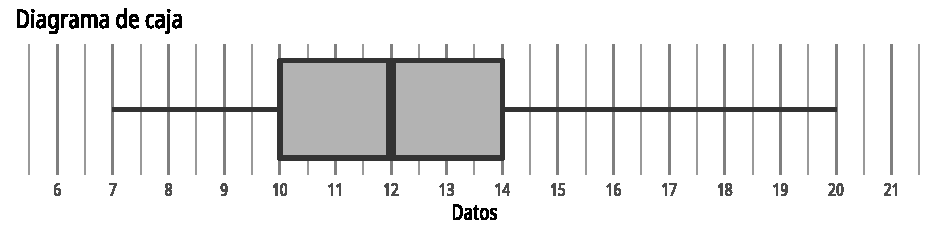
\includegraphics{diagrama_caja_2.pdf}\end{center}
\end{document}
